\chapter{Optical Character Recognition}
\label{chap:ocr}

In this chapter, we summarize existing \gls{ocr} methods and describe the two methods we use in this thesis, EasyOCR and Tesseract \gls{ocr}, in detail.
We also introduce the \gls{cer} metric, which we use to evaluate the \gls{ocr} methods.

\section{Conventional Optical Character Recognition}

\Gls{ocr} \cite{ocr_survey_2017} generally involves the following steps to extract text from an image.
First, the images are preprocessed, which might include binarization, noise removal, and skew correction.
This step tries to improve the quality of the image from the perspective of the \gls{ocr} method.
Second, the image is segmented into individual characters, words or lines.
Next, the segmented elements are categorized by Bayesian, nearest neighbor or neural network based classifiers.
Finally, the recognized elements are postprocessed, which might include the use of multiple classifiers simultaneously and comparison of the results, incorporation of the context of the image or dictionary data to correct errors.

\section{Neural Network Based Optical Character Recognition}

In recent years, classifiers based on neural network based methods \cite{ocr_survey_lstms_2013} have become more popular.
Especially \gls{lstm} networks are prominent.
In general, neural network based methods perform better than conventional methods.

Some of the most popular examples is Calamari \cite{ocr_calamari_2018}, which is focused on recognizing text in historical documents.
It uses the \gls{ctc} method to train a model composed of \gls{lstm} and \gls{cnn} layers.
This leads to state of the art performance on historical document datasets.

Another example is the Inception V3 network \cite{ocr_improved_deep_2018}, which implements a \gls{cnn} to recognize printed text in images with poor quality.
The deep learning method shows significant improvements over traditional \gls{ocr} methods, especially for low quality images.

The \gls{ocr} methods used in this thesis, EasyOCR and Tesseract, are described in the following sections.

\section{EasyOCR}
\label{subsec:easyocr}

\begin{figure}[h!]
    \centering
    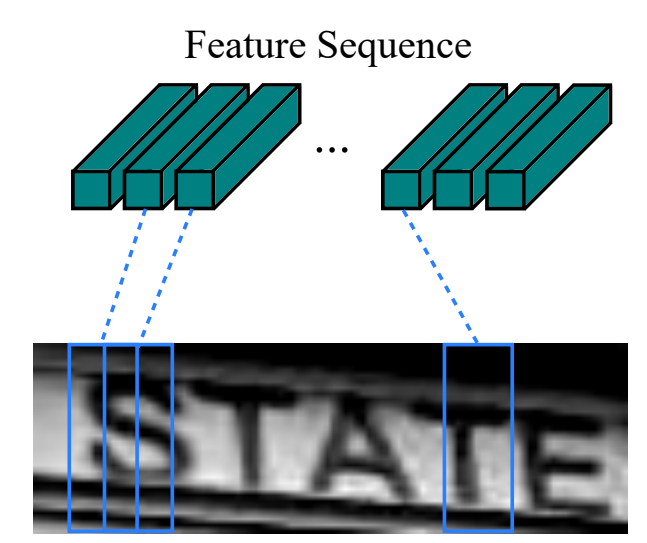
\includegraphics[width=0.5\textwidth]{../images/external/crnn_features.png}
    \caption{EasyOCR feature sequencing for an image of the word \texttt{state}, from \cite{easyocr_2020}.}
    \label{fig:easyocr_features}
\end{figure}

EasyOCR is an open source Python library for \gls{ocr} \cite{easyocr_gitub_2020}.
It leverages the CRAFT algorithm \cite{craft_2019} for text detection, utilizing a fully convolutional network structure to predict word or character boxes within an image.
For text recognition, EasyOCR adopts the None-VGG-BiLSTM-CTC architecture \cite{crnn_2015}.

For the recognition task, the model consists of convolutional layers to extract relevant features from the input image.
These features are then transformed into sequences, as illustrated in \autoref{fig:easyocr_features}.
Then, a deep bidirectional \gls{lstm} network is used to predict a character per frame of the feature sequence.
This process generates output that may resemble something like \texttt{--ss-t-a-tt--e-}.
The benefit of using the \gls{lstm} lies in its ability to incorporate contextual information from earlier frames of the sequence to enhance the recognition accuracy.
Finally, the transcription layer uses \gls{ctc} to combine the per-frame predictions into a single text prediction, for instance, generating the word \texttt{state}.
Optionally, this text prediction can be compared to a lexicon, which allows for additional validation and refinement.
This comparison ensures that the recognized text aligns with known words or patterns, enhancing the accuracy and reliability of the OCR results.
Throughout this thesis, we rely on version v1.6.2 of EasyOCR.


\section{Tesseract}
\label{subsec:tesseract}

The second \gls{ocr} method we utilize in this thesis is Tesseract \gls{ocr} \cite{tesseract_legacy_2007}\cite{tesseract_github_2023}\cite{tesseract_architecture_2016}.
Originally developed by Hewlett-Packard in the 1980s, it was open sourced in 2005 and subsequently developed by Google from 2006 to 2018.
Tesseract \gls{ocr} employs adaptive thresholding to binarize the input image, enhancing the contrast between text and background.
Following this step, the software performs page layout analysis to identify text regions within the image.
These regions are then processed by the \gls{lstm} line recognizer to generate text predictions.
Finally, the text prediction undergo correction measures to improve the accuracy of the result.

To our knowledge, the literature on Tesseract \gls{ocr} focuses on older versions of the software, predating the introduction of \gls{lstm} models with version 4.0.0.
Consequently, detailed information about the \gls{lstm} line recognizer is not available.
For our experiments in this thesis, we rely on version 4.1.1 of Tesseract \gls{ocr}.
Due to Tesseract \gls{ocr} being implemented in C++, we utilize the Python wrapper, \texttt{pytesseract} \cite{pytesseract_2022}, to conveniently incorporate it into our Python code.
To ensure a fair comparison, we do not preprocess the images for either \gls{ocr} method, as we are unsure of the specific preprocessing steps employed by each method itself and wish to avoid any potential bias.
For text prediction, we use the default settings for EasyOCR and Tesseract \gls{ocr}.
Comparative research between EasyOCR and Tesseract \gls{ocr}, specifically in the task of recognizing text in license plate images \cite{ocr_tess_vs_easyocr_2022}, indicates that EasyOCR generally outperforms Tesseract \gls{ocr}.

% --- connection threshold of boundingbox, difficult to set correctly, cant use dict if single letters, auto puts sentences together when high


\section{Character Error Rate}
\label{subsec:cer}

To evaluate the performance of \gls{ocr} methods, we use the \gls{cer}.
The \gls{cer} \cite{cer_2022} describes how many substitutions, deletions, and insertions are necessary to transform a text prediction into the text label.
It is defined as

\begin{equation}
    \text{CER} = \frac{I + S + D}{N},
    \label{eq:cer}
\end{equation}

with $I$ being the number of insertions, $S$ being the number of substitutions, $D$ being the number of deletions, and $N$ being the total number of characters in the text label.
The \gls{cer} ranges from 0 to $\infty$, where 0 means perfect recognition and the higher the worse the recognition.
As an example, if the text label is \texttt{hello} and the prediction is \texttt{halo}, then the \gls{cer} is $2/5 = 0.2$, due to one insertion (\texttt{l}) and one substitution (\texttt{a $\rightarrow$ e}).

In our analysis, we will be comparing the \gls{cer} to the subjective \gls{mos}.
The details of the subjective \gls{mos} will be discussed in the following chapter.
Because the \gls{mos} is defined in the range 0 to 100 and 100 represents a high subjective quality, the two metrics are unintuitive to compare.
Therefore, we take the complement of the CER by subtracting it from 1.
Additionally we scale it by multiplying by 100 to get a \gls{mos}-like value, according to

\begin{equation}
    \text{CER}_{\text{c}} = (1 - \text{CER}) \cdot 100.
    \label{eq:cer2mos}
\end{equation}

This means that the $\text{CER}_{\text{c}}$ can be in the range -$\infty$ to 100, where 100 means perfect recognition and the lower the worse the recognition.
However, in practice, the $\text{CER}_{\text{c}}$ typically falls within the range of 0 to 100, which aligns with the scale of the \gls{mos}.
This can be illustrated by a few examples.
Let's consider the text label as \texttt{hello} and the prediction as empty.
In this case, the \gls{cer} would be $5/5 = 1$, as there are 5 insertions necessary to match the text label, and the $\text{CER}_{\text{c}}$ would be $0$.
Thus, if the prediction is shorter than the text label, the $\text{CER}_{\text{c}}$ cannot be negative.
The only scenario where a negative $\text{CER}_{\text{c}}$ can be obtained is if the prediction is longer than the text label and the prediction is incorrect.
For instance, if the text label is \texttt{hello} and the prediction is \texttt{goodbye}, the \gls{cer} would be $7/5 = 1.4$, as there are 5 substitutions and 2 deletions required to match the text label, resulting in a negative $\text{CER}_{\text{c}}$ of $-40$.
However, this case is highly unlikely, because the \gls{ocr} methods incorporate a confidence threshold, which means that they refrain from predicting a word if they lack confidence in its correctness.
Therefore, the word predictions are either empty, making the whole prediction shorter than the text label, or they have a high likelihood of being correct.

In order to apply the \gls{ocr} methods discussed in this chapter, a suitable dataset comprising images containing text is essential.
Thus, in the following chapter, we provide an overview of the available datasets and present the dataset employed in this thesis in detail.
